%%%%%%%%%%%%%%%%%%%%%%%%%%%%%%%%%%%%%%%%%%%%%%%%%%%%%%%%%%%%%%%%%
\clearpage
\chapter{UPCOMING WORK}\label{Ch6}
%%%%%%%%%%%%%%%%%%%%%%%%%%%%%%%%%%%%%%%%%%%%%%%%%%%%%%%%%%%%%%%%%
\section{Instructions to be Added}
After experimenting with MLA instruction, we were given a new hardware target which lacked support in LLVM \cite{eryilmaz}. The hardware is based on the RISC-V instruction set extended by rotation (ROT) and s-box which is specific to the ASCON encryption algorithm the hardware aims to accelerate. 
\par
\subsection{ROT/ROTI Instruction}
Due to complications in LLVM at representing circular shift instead of linear shift at IR level, a new intrinsic function funnel shift (llvm.fshl) was introduced to the codebase. To see if it is generated at the assembly level, it is a better practice to declare the function in the .ll file that is fed into LLC program. As ROT is a more popular instruction to be extended LLVM may have support already through for example the bit manipulation extension and moreover the ways to enable it will be investigated. 

\subsection{S-BOX Instruction}
 
\begin{figure}
    \centering
    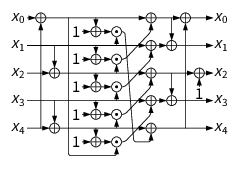
\includegraphics{upcoming_work/s_box_ascon.png}
    \caption{S-Box Layer of ASCON}
    \label{fig:sbox}
\end{figure}
S-Box instruction used in the ASCON algorithm is a series of XORs and ORs between bits of 5 words which can be seen in Figure \ref{fig:sbox}. The instruction is hard to generalize and the hardware implementation is implementing the instruction as from memory to memory which poses another set of challenges for us to overcome.
\section{Hardware Modifications}
The ROT instruction is implemented on hardware however the immediate version of it, ROTI, is not. After implementing the ROT instruction at LLVM we will try to modify the hardware without harming its integrity.
